% License:
% CC BY-NC-SA 3.0 (http://creativecommons.org/licenses/by-nc-sa/3.0/)
%----------------------------------------------------------------------------------------
%	PACKAGES AND OTHER DOCUMENT CONFIGURATIONS
%----------------------------------------------------------------------------------------
\documentclass[paper=letter, fontsize=12pt]{scrartcl} % A4 paper and 11pt font size
\usepackage[margin=1in]{geometry}
\usepackage[T1]{fontenc} % Use 8-bit encoding that has 256 glyphs
\usepackage[english]{babel} % English language/hyphenation
\usepackage{sectsty} % Allows customizing section commands
\allsectionsfont{\centering \normalfont\scshape} % Make all sections centered, the default font and small caps
\usepackage{amsmath}
\usepackage{fancyhdr} % Custom headers and footers
\pagestyle{fancyplain} % Makes all pages in the document conform to the custom headers and footers
\fancyhead{} % No page header - if you want one, create it in the same way as the footers below
\fancyfoot[L]{} % Empty left footer
\fancyfoot[C]{\thepage} % Empty center footer
\fancyfoot[R]{} % Page numbering for right footer
\renewcommand{\headrulewidth}{0pt} % Remove header underlines
\renewcommand{\footrulewidth}{0pt} % Remove footer underlines
\setlength{\headheight}{13.6pt} % Customize the height of the header
\usepackage{graphicx}
\usepackage{wrapfig}
\usepackage{hyperref}
\usepackage{setspace}
\usepackage{color}
%\doublespacing

%----------------------------------------------------------------------------------------
%	TITLE SECTION
%----------------------------------------------------------------------------------------

\newcommand{\horrule}[1]{\rule{\linewidth}{#1}} % Create horizontal rule command with 1 argument of height

\title{	
\normalfont \normalsize 
\textsc{Working Draft for Hindsight Conference\\APA New York Metro Chapter Diversity Committee\\November 2, 2018} \\ [6pt] % Your university, school and/or department name(s)
\horrule{1pt} \\[0.5cm] % Thin top horizontal rule
\huge Measuring the Impacts of Redlining\\% The assignment title
\horrule{1pt}\\[0.5cm] % Thick bottom horizontal rule
}
\author{Addison Larson} % Your name
\date{\normalsize{\today}} % Today's date or a custom date

\begin{document}

\maketitle % Print the title
\newpage
\tableofcontents
\newcommand{\blankpage}{
	\newpage
	%\thispagestyle{empty}
	\mbox{}
	\newpage
}
\listoftables
\blankpage
% ----------------------------------
% START PAPER
% ----------------------------------
\section{Introduction}
Zoning and housing policy have been tools of discrimination. The first zoning ordinances from the early 1900s were explicitly designed for racial exclusion. Housing discrimination has persisted ever since, from the practice of redlining to the subprime lending crisis \cite{rothstein}.\par
By studying digitized redlining maps from the Home Owners' Loan Corporation (HOLC), data on job accessibility via transit, and Census estimates across 17 U.S. metropolitan areas, this project quantifies the impacts of redlining on today's urban landscape. A one-point decrease in HOLC rating corresponds to the following modern-day effects: 
\begin{enumerate}
	\item \textbf{\$62,175 decrease} in median home value, controlling for size, age, and facilities;
	\item \textbf{13.962\% decrease} in homeownership;
	\item \textbf{2.794\% increase} in rent burden;
	\item \textbf{25,185 additional jobs} accessible via transit;
	\item \textbf{10.869\% increase} in transit-dependent households;
	\item \textbf{\$3,107 decrease} in annual household income, controlling for education levels; and
	\item \textbf{10.659\% increase} in household poverty.
\end{enumerate}
Many neighborhoods remain racially segregated as they were during HOLC's operation from the 1930s to the 1950s. \textbf{Today, Black residents are 15.153\% more likely, and white residents 16.806\% less likely, to live in a census tract once downgraded by HOLC.}

An absence of racially discriminatory housing policies has \textit{not} translated into equity in terms of accessing education or building wealth. If we take equity seriously, we must emphasize proactive and progressive housing policies. 

\section{Problem Statement and Project Objective}
This study is based on three premises:
\begin{enumerate}
	\item Cities in the U.S. are racially segregated.
	\item Racially discriminatory housing policies have facilitated segregation in cities.
	\item The location of one's home sets the stage for one's future prospects, including access to a quality education; workforce preparedness; and access to jobs for which one is qualified. These factors affect one's ability to earn an income and accumulate wealth over time.
\end{enumerate}

\subsection{Racial Segregation in U.S. Cities}
\textbf{Cities in the U.S. are racially segregated.} I think it would be useful to calculate indices of dissimilarity for the cities in your study area. Take this time also to explain what the index of dissimilarity means, what the minimum and maximum are, and to cite the authors who came up with it.\par

\begin{table}[h]
	\caption{Indices of Black-White Dissimilarity for 17 U.S. Metro Areas}
	\begin{center}
		\begin{tabular}{||l | c||}
			\hline
			\textbf{Metropolitan Statistical Area} & \textbf{D\textsubscript{I}} \\
			\hline \hline
			Atlanta, GA & 0.560 \\
			\hline
			Baltimore, MD & 0.626 \\
			\hline
			Birmingham, AL & 0.649 \\
			\hline
			Buffalo-Niagara Falls, NY & 0.708 \\
			\hline
			Charlotte-Gastonia-Rock Hill, NC-SC & 0.505 \\
			\hline
			Columbus, OH & 0.600 \\
			\hline
			Indianapolis, IN & 0.627 \\
			\hline
			Kansas City, MO-KS & 0.574 \\
			\hline
			Louisville, KY-IN & 0.568 \\
			\hline
			Minneapolis-St. Paul, MN-WI & 0.542 \\
			\hline
			New Orleans, LA & 0.631 \\
			\hline
			Norfolk-Virginia Beach-Newport News, VA-NC & 0.472 \\
			\hline
			Pittsburgh, PA & 0.657 \\
			\hline
			Portland-Vancouver, OR-WA & 0.488 \\
			\hline
			San Diego, CA & 0.441 \\
			\hline
			St. Louis, MO-IL & 0.709 \\
			\hline
			Tampa-St. Petersburg-Clearwater, FL & 0.511 \\
			\hline
		\end{tabular}
	\end{center}
Author's calculations from 2016 ACS 5-Year Estimates, Table B02001.
\end{table}

\subsection{Housing Policy and Racial Segregation}
\textbf{Racially discriminatory housing policies have facilitated segregation in cities.} From the 1930s to the 1950s, the Home Owners' Loan Corporation (HOLC) provided Americans the opportunity to purchase homes through mortgage lending. However, this federally-created program was racially discriminatory in its administration. HOLC created color-coded maps of U.S. cities, grading neighborhoods along a four-point scale from \textit{A} to \textit{D}. Applications to purchase homes in green neighborhoods --- ``Class A'' --- were nearly guaranteed approval; applications to purchase homes in red neighborhoods --- ``Class D'' --- were subject to immediate denial. ``Class A'' neighborhoods were all-white neighborhoods; ``Class D'' neighborhoods were all-Black neighborhoods. HOLC lending practices gave birth to the term ``redlining,'' after those neighborhoods downgraded by the agency.\par

HOLC lending practices were as biased in their effects as in their administration. First, redlining enforced racial segregation in cities, because it encouraged white residents to purchase homes in all-white neighborhoods and prevented Black residents from moving into these neighborhoods. Second, redlining encouraged a divergence in wealth between Black and white residents. White residents received a generous opportunity to build generational wealth. Meanwhile, Black residents were systematically discriminated against in the housing market, forced to pay exorbitant prices for substandard rental housing, and barred from the chance to buy homes and invest in their futures. HOLC redlining is but one example among a legacy of racially discriminatory housing policies.\cite{rothstein}\par

\subsection{Home as a Platform for (Dis)Opportunity}
\textbf{The location of one's home sets the stage for one's future prospects, including access to a quality education; workforce preparedness; and access to jobs for which one is qualified. These factors affect one's ability to earn an income and accumulate wealth over time.} Mention and cite a few examples, including the Geography of Opportunity, job search theory, and Raj Chetty.\par

\subsection{Project Objective}
Recognizing the role of racial segregation in housing and the effects of home location on education, income, and wealth, this project has two aims: first, to \textbf{quantify the impact of HOLC redlining} on education, work, income, and wealth today; and second, to \textbf{evaluate redlining's disparate and lingering racial effects} between Black and white residents.\par

\section{Hypothesized Relationships}
\subsection{Hypotheses}
\begin{enumerate}
	\item \textbf{Access to Education:} Current educational attainment will be lower in downgraded HOLC neighborhoods.
	\item \textbf{Access to Jobs via Transit:} Because downgraded HOLC neighborhoods are typically located close to the city center, more jobs will be accessible via transit.
	\item \textbf{Wealth Creation:} Current incomes, home value, and homeownership will be lower in downgraded HOLC neighborhoods; poverty, unemployment, and rental burdens will be higher.
\end{enumerate}
\subsection{Variable Selection and Expectation}
Notes if necessary.\par
\begin{enumerate}
	\item \textbf{Educational Attainment}\\
	\textit{Description:} The percentage of residents who have completed the following: 1) high school diploma or its equivalent; 2) some college; 3) four-year degree; and 4) graduate or professional degrees. (All measures at the census tract level.)\\
	\textit{Expected Relation to HOLC redlining:} As the HOLC neighborhood score decreases:
	\begin{enumerate}
		\item The percentage of residents with a high school diploma or its equivalent will increase;
		\item The percentage of residents with some college will increase;
		\item The percentage of residents with a four-year degree will decrease; and
		\item The percentage of residents with a graduate or professional degree will decrease.
	\end{enumerate}
	
	\item \textbf{Access to Jobs via Transit}\\
	\textit{Description:} The number of jobs accessible within 30 minutes of a census tract using transit. (All measures at the census tract level.)\\
	\textit{Expected Relation to HOLC redlining:} As the HOLC neighborhood score decreases, the access to jobs via transit will increase, because redlined neighborhoods, transit service, and jobs are concentrated in the urban core.
	
	\item \textbf{Wealth Creation}\\
	\textit{Description:} 1) Median household income, with educational attainment as a control factor. 2) The percentage of owner-occupied housing units. 3) Median home value, with housing age, size, and facilities as control factors. 4) Percentage of households below 100\% and 150\% of the Federal Poverty Level (FPL) respectively. 5) Percentage of unemployed residents in the labor force. 6) Median gross rent as a percentage of annual income. (All measures at the census tract level.)\\
	\textit{Expected Relation to HOLC redlining:} As the HOLC neighborhood score decreases:
	\begin{enumerate}
		\item Median household income will decrease;
		\item The percentage of owner-occupied housing units will decrease;
		\item Median home value will decrease;
		\item The percentage of households in poverty will increase;
		\item The percentage of unemployed residents will increase; and
		\item Renters will spend a larger percent of their income on rent.
	\end{enumerate}
\end{enumerate}

\section{Study Area, Data Sources, and Methodology}
\subsection{Study Area}
Two of the data sources used in this study are limited in their geographic coverage. First, the University of Richmond's ``Mapping Inequality'' project has digitized HOLC redlining maps for 128 cities. Some of the digitized maps do not fall within MSAs (e.g. Durham, NC) and others must be merged together to better correspond to one MSA (e.g. St. Louis, MO and East St. Louis, IL). This results in fewer than 128 potential study areas. Second, the University of Minnesota's ``Access Across America'' project has computed job accessibility by transit for 46 of the 50 largest metro areas. Any MSAs with areas present in both the HOLC redlining maps and the job accessibility files were included in the study area (see Figure 1).\par
\begin{figure}[h]
	\centering
	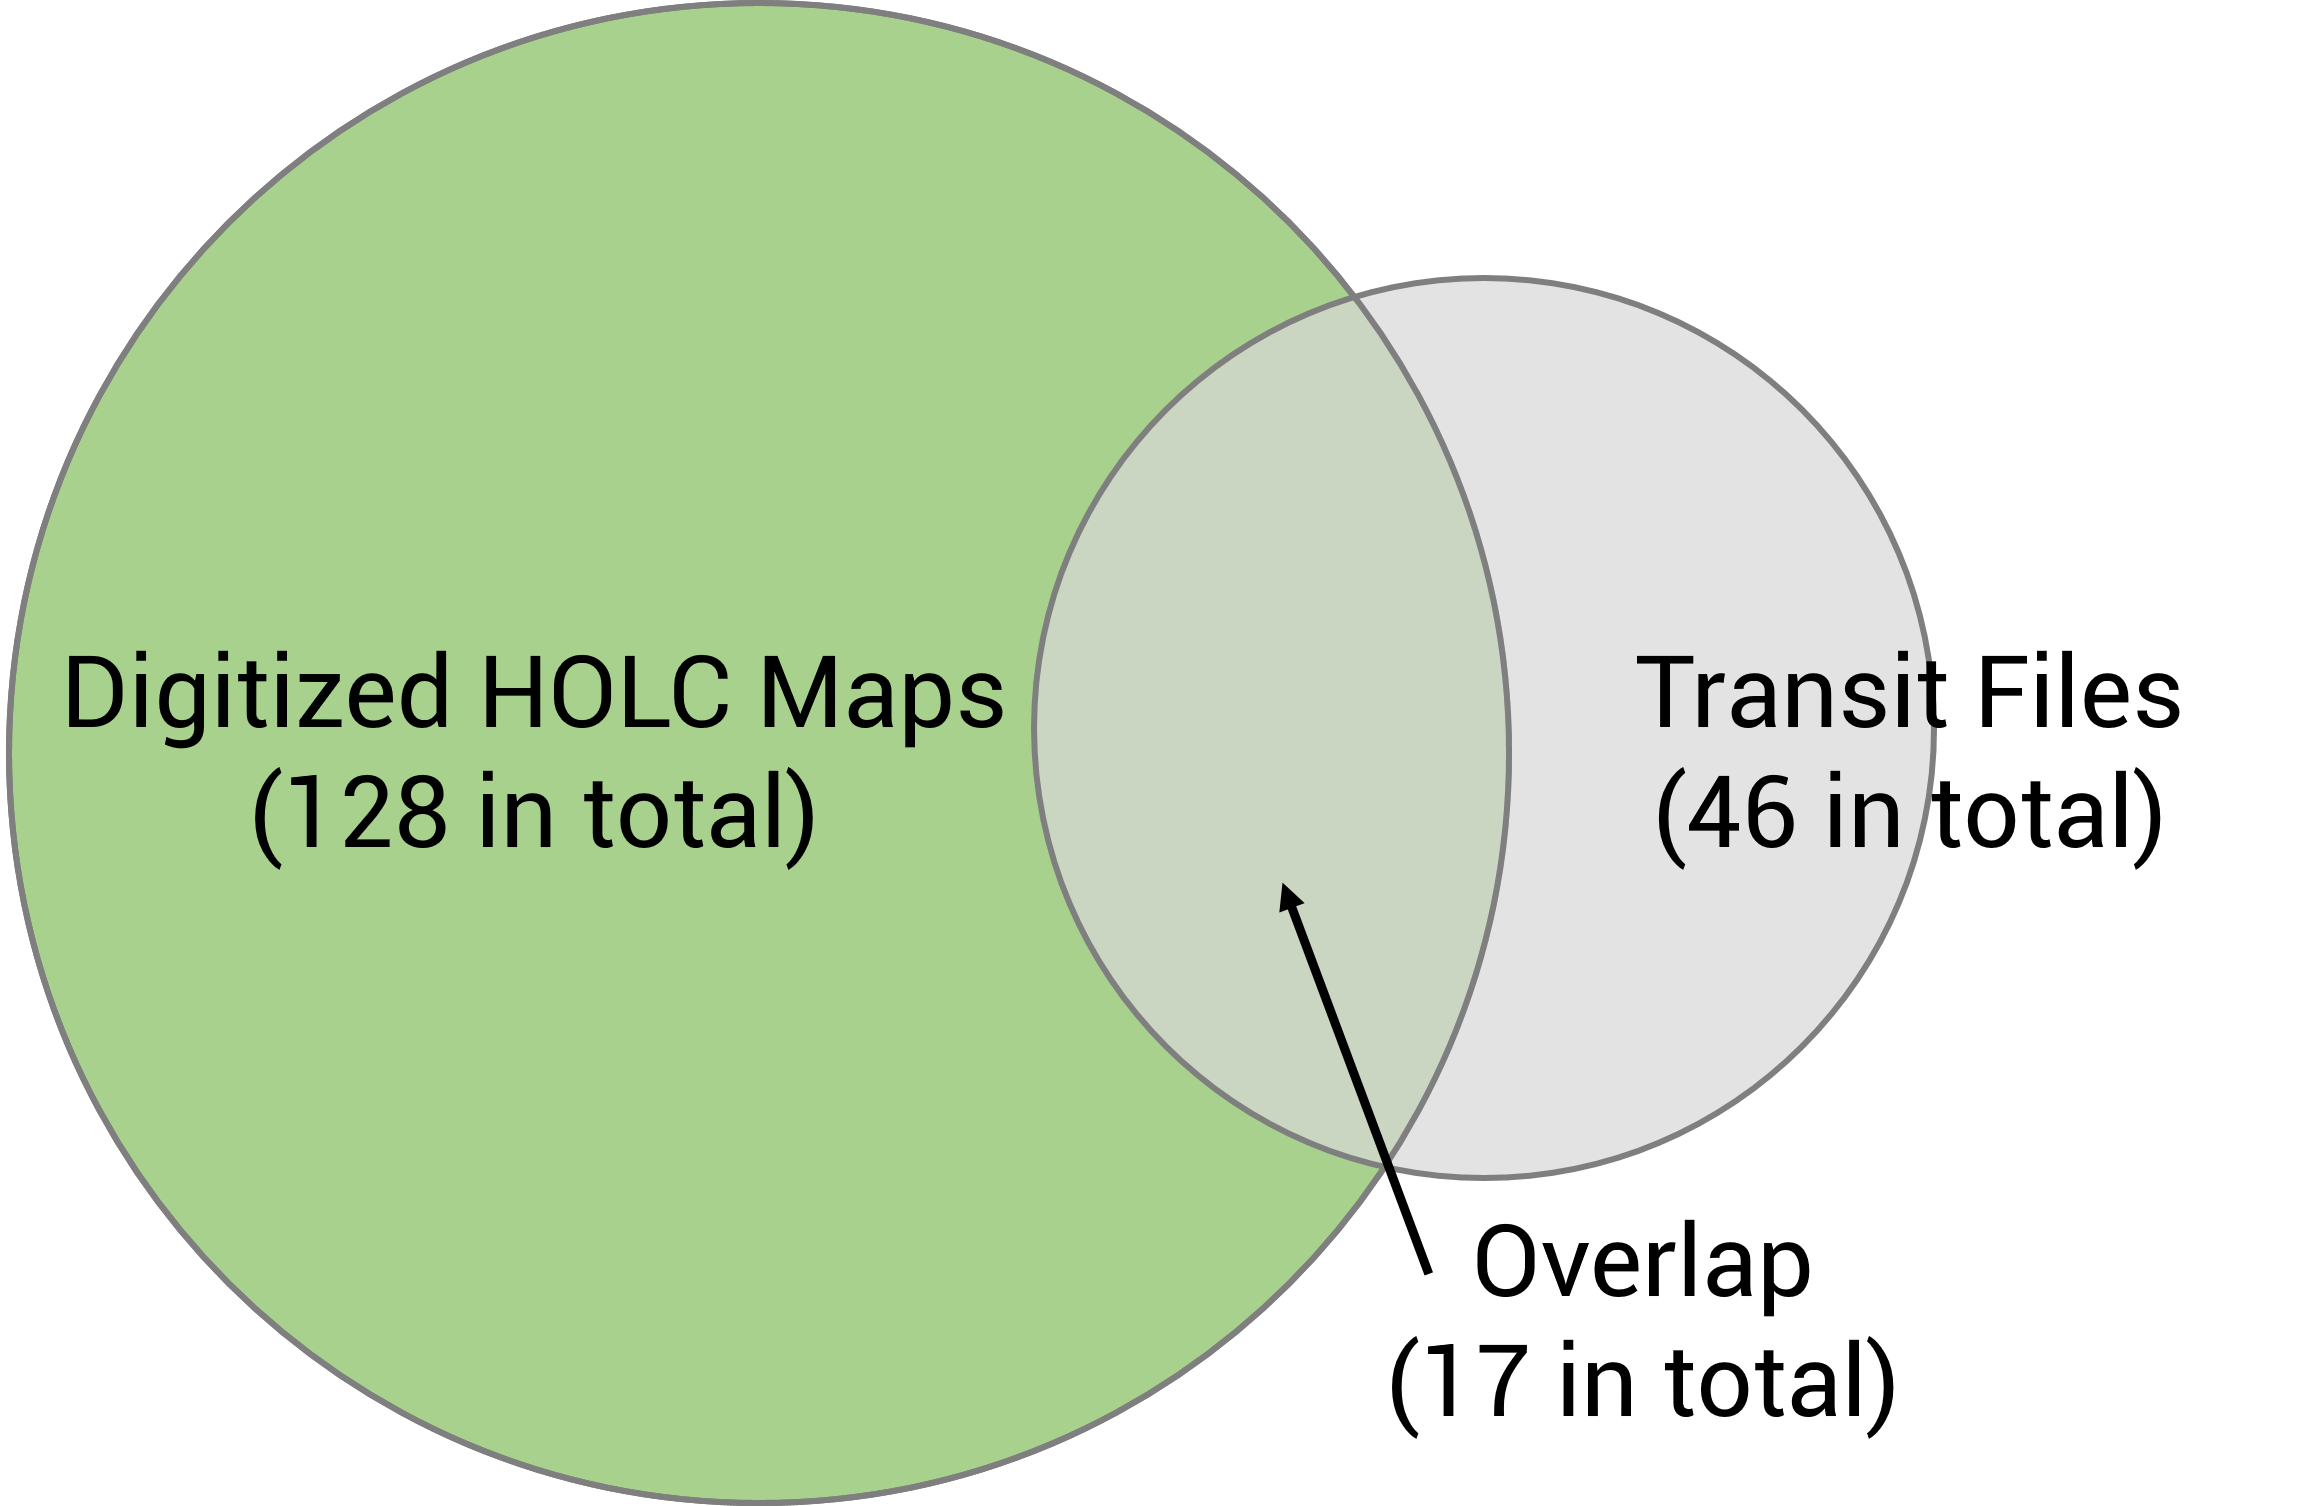
\includegraphics[width = 4.5in]{StudyAreaSelection}\\
	\caption{All MSAs present in both the digitized HOLC maps and in the transit accessibility files were included in the project.}
\end{figure}
These MSAs include: Birmingham, AL; San Diego, CA; Tampa-St. Petersburg-Clearwater, FL; Atlanta, GA; St. Louis, MO-IL; Indianapolis, IN; Kansas City, MO-KS; Louisville, KY-IN; New Orleans, LA; Baltimore, MD; Minneapolis-St. Paul, MN; Buffalo-Niagara Falls, NY; Charlotte-Gastonia-Rock Hill, NC-SC; Columbus, OH; Portland-Vancouver, OR-WA; Pittsburgh, PA; and Norfolk-Virginia Beach-Newport News, VA-NC.
\subsection{Data Sources and Methodology}
This project utilizes four primary sources of information:
\begin{enumerate}
	\item \textbf{Shapefiles from the Census Bureau's Topologically Integrated Geographic Encoding and Referencing (TIGER/Line) collection.} \cite{tiger17}\\
	TIGER/Line shapefiles are available for every state at the census tract level. Because some MSAs cross state borders, 21 state shapefiles were used, including AL, CA, FL, GA, IL, IN, KS, KY, LA, MD, MN, MO, NC, NY, OH, OR, PA, SC, VA, WA, and WI. These files were subset by \textit{GEOID} to match the spatial extent of MSAs, and census tracts outside MSA boundaries were removed from the files.
	\item \textbf{Digitized Shapefiles of HOLC Maps from the University of Richmond's Digital Scholarship Lab.} CITE!!!! \\
	The University of Richmond's ``Mapping Inequality'' project has digitized HOLC maps from 128 cities and towns. These shapefiles trace over the boundaries of HOLC neighborhoods and include the neighborhood grade as an attribute. Historic HOLC neighborhood boundaries do not align with present-day census tract boundaries. As an approximation of HOLC rating at the census tract level, each HOLC rating is assigned a numeric value (``Class A'' = 4; ``Class D'' = 1). A union operation is performed in GIS with all census tract shapefiles at the MSA level. The union produces three scenarios, which are handled in statistical software:
	\begin{enumerate}
		\item When a unique \textit{GEOID} is associated with only one HOLC rating, it is given that rating. These cases occur when the HOLC neighborhood encompasses the entire census tract or when the census tract is located on the periphery of the historic HOLC map.
		\item When a unique \textit{GEOID} is associated with multiple HOLC ratings, it is assigned the mean of these ratings. Note that this methodology is imperfect and does not account for the area of overlap. One way to account for the area of overlap is to rasterize both the census tract and HOLC rating shapefiles and then to compute the mean HOLC rating by \textit{GEOID}.
		\item When a unique \textit{GEOID} is not associated with any HOLC rating, it is given the value \texttt{NA}. These cases typically occur when the MSA falls outside the periphery of the historic HOLC map or when the MSA is located in the Central Business District.
	\end{enumerate}
	\item \textbf{Job Accessibility Files from the University of Minnesota's \textit{Access Across America: Transit 2014} Study.} CITE!!!! \\
	Include description here. Discuss collapse. Brief overview on how and why you collapse the transit accessibility files.
	\item \textbf{Demographic and Commuting Characteristics from the Census Bureau's 2016 American Community Survey (ACS) 5-Year Estimates.} \cite{acs16}\\
\end{enumerate}
While all data is available at the city or MSA level, the main point of interest is in national trends. We cannot assume that observations within a city are independent of one another; an inherent hierarchical structure is present in the data. Therefore, multilevel modeling is a preferred analysis approach to OLS. Fixed-coefficient, random-slope multilevel models are used, essentially allowing to control for effects by city.

\section{Results}
\begin{table}
	\caption{Summary of Census Tract Characteristics by HOLC Rating}
	\begin{center}
		\begin{tabular}{|| l | c c c c ||}
			\hline
			Variable & Class A & Class B & Class C & Class D \\
			\hline \hline
			Number of Observations & 5 & 60 & 188 & 140\\
			\hline 
			Avg. Tract Population & 3,680 & 3,222 & 2,974 & 2,490\\
			\hline 
			\multicolumn{5}{|| c ||}{Housing}\\
			\hline 
			Median Home Value, 1000s & \$371.3 & \$250.33 & \$159.09 & \$145.08\\
			\hline 
			Pct. Owner-Occupied Housing Units & 82.52 & 57.33 & 39.78 & 34.38\\
			\hline 
			Median Home Age, Years & 79 & 74.4 & 69.36 & 66.72\\
			\hline 
			Median Monthly Rent & \$1,103 & \$999 & \$864 & \$814\\
			\hline 
			Median Gross Rent as \% of Ann. Inc. (GRAPI) & 27.3 & 30.05 & 34.9 & 37.1\\
			\hline 
			\multicolumn{5}{|| c ||}{Job Access}\\
			\hline 
			No. Jobs Accessible by Transit & 36,977 & 51,054 & 56,020 & 82,190\\
			\hline 
			Pct. Zero-Car Households & 2.7 & 13.98 & 22.2 & 31.77\\
			\hline 
			Pct. Unemployed in Labor Force & 3.52 & 7.58 & 12.34 & 14.65\\
			\hline 
			\multicolumn{5}{|| c ||}{Income and Poverty Trends}\\
			\hline 
			Annual Median Household Income & \$50,849 & \$34,640 & \$23,236 & \$19,542\\
			\hline 
			Pct. Households Below 150\% FPL & 1.74 & 6.88 & 14.18 & 17.78\\
			\hline 
			Pct. Households Below 100\% FPL & 2.65 & 6.28 & 10.77 & 12.66\\
			\hline 
			Pct. Single-Parent Households & 7.99 & 16.39 & 25.88 & 28.82\\
			\hline 
			\multicolumn{5}{|| c ||}{Education}\\
			\hline 
			Pct. HS Degree or Equivalent & 7.56 & 18.56 & 26.5 & 29.26\\
			\hline 
			Pct. Some College, No Degree & 12.24 & 17.16 & 21.23 & 19.43\\
			\hline 
			Pct. 4-Year College Degree & 37.83 & 26.3 & 17.82 & 12.65\\
			\hline 
			Pct. Grad./Prof. Degree & 35.35 & 22.46 & 11.28 & 8.42\\
			\hline 
			\multicolumn{5}{|| c ||}{Race \& Ethnicity}\\
			\hline 
			Pct. White Residents & 88.45 & 62.85 & 43.05 & 33.6\\
			\hline 
			Pct. Black Residents & 4.15 & 28.03 & 45.8 & 55.69\\
			\hline 
			Pct. Asian Residents & 3.51 & 3.5 & 3.68 & 2.57\\
			\hline 
			Pct. Hispanic Residents & 2.39 & 5.71 & 10.32 & 15.44\\
			\hline 
			Pct. Majority-White Tracts & 100 & 75 & 47 & 29\\
			\hline 
			Pct. Majority-Black Tracts & 0 & 25 & 47 & 61\\
			\hline 
			Pct. Majority-Asian Tracts & 0 & 0 & 1 & 0\\
			\hline 
			Pct. Majority-Hispanic Tracts & 0 & 0 & 4 & 10\\
			\hline 
		\end{tabular}
	\end{center}
	Author's calculations from the following: \textit{(1)} Nelson, R.K., \& Ayers, E.L., eds. (n.d.). ``Mapping Inequality.'' \textit{American Panorama}. Accessed August 25, 2018. \textit{(2)} Owen, A., \& Levinson, D.M. (2014). \textit{Access Across America: Transit 2014 Data}. Retrieved from the Data Repository for the University of Minnesota, \href{http://dx.doi.org/10.13020/D6MW2Q}{http://dx.doi.org/10.13020/D6MW2Q}. \textit{(3)} 2016 ACS 5-Year Estimates, Tables B01001, B06011, B08122, B02001, B03001, B25064, B25077, B25035, B25003, B25041, B25048, B25051, B23025, B15003, B08201, B25071, and B11001.
\end{table}

\begin{table}
	\textbf{HOLC Rating and Home Value.} A one-point decrease in HOLC rating corresponds to a \$62,175 decrease in median home value, controlling for housing unit size, age, and facilities. Interestingly, there is a negative relationship between median home values and housing unit size: census tracts with higher percentages of larger homes are associated with lower home values. This may be because smaller homes are more frequently located in the city center, where housing costs are the highest. Going forward, a more reliable method will use appraisal data to relate home value to HOLC rating and control by housing unit characteristics at the parcel level.
	\caption{Multilevel Model: Home Value, \$1000s}
	\begin{center}
		\begin{tabular}{|| l | c c c ||}
			\hline
			Variable & $\beta$ & SE & \textit{p} \\
			\hline \hline
			Intercept & -172.806 & 486.170 & 0.722 \\
			\hline
			HOLC Score & 62.175 & 7.545 & 0.001*** \\
			\hline
			0 Bedrooms & -3.235 & 1.911 & 0.091* \\
			\hline
			1 Bedroom & -4.339 & 1.404 & 0.002*** \\
			\hline
			2 Bedrooms & -5.768 & 1.332 & 0.001*** \\
			\hline
			3 Bedrooms & -7.101 & 1.374 & 0.001*** \\
			\hline
			4 Bedrooms & -2.787 & 1.869 & 0.137 \\
			\hline
			Age of Home & 0.474 & 0.404 & 0.241 \\
			\hline
			Complete Plumbing Facilities & 9.436 & 4.549 & 0.039** \\
			\hline
			Complete Kitchen Facilities & -2.021 & 0.540 & 0.001*** \\
			\hline
			Birmingham, AL & 94.098 & 91.656 & 0.305 \\
			\hline
			San Diego, CA & 209.557 & 86.443 & 0.016** \\
			\hline
			Tampa, FL & 15.954 & 91.818 & 0.862 \\
			\hline
			Atlanta, GA & 154.585 & 98.984 & 0.119 \\
			\hline
			St. Louis, MO & -75.060 & 86.462 & 0.386 \\
			\hline
			Indianapolis, IN & -18.228 & 85.483 & 0.831 \\
			\hline
			Kansas City, MO & -50.450 & 86.560 & 0.560 \\
			\hline
			Louisville, KY & -64.334 & 88.052 & 0.465 \\
			\hline
			New Orleans, LA & 132.570 & 86.993 & 0.128 \\
			\hline
			Baltimore, MD & 14.845 & 86.299 & 0.864 \\
			\hline
			Minneapolis, MN & -22.681 & 85.886 & 0.792 \\
			\hline
			Buffalo, NY & -70.195 & 90.658 & 0.439 \\
			\hline
			Charlotte, NC & 114.962 & 95.065 & 0.227 \\
			\hline
			Columbus, OH & -12.475 & 89.531 & 0.889 \\
			\hline
			Portland, OR & 81.021 & 128.403 & 0.528 \\
			\hline
			Pittsburgh, PA & -48.048 & 86.774 & 0.580 \\
			\hline
			Norfolk, VA & NA & NA & NA \\
			\hline
		\end{tabular}
	\end{center}
\textit{SE} = 84.05 on 361 degrees of freedom. \textit{Adj. R\textsuperscript{2}} = 0.587. \textit{F} = 22.96 on 25 and 361 degrees of freedom, \textit{p} = 0.001. Norfolk, VA Boolean variable is removed because of multicollinearity.\\
Author's calculations from the following: \textit{(1)} Nelson, R.K., \& Ayers, E.L., eds. (n.d.). ``Mapping Inequality.'' \textit{American Panorama}. Accessed August 25, 2018. \textit{(2)} 2016 ACS 5-Year Estimates, Tables B25035, B25041, B25048, B25051, and B25077.
\end{table}

\begin{table}
	\textbf{HOLC Rating and Home Ownership.} A one-point decrease in HOLC rating corresponds to a 13.962\% decrease in home ownership.
	\caption{Multilevel Model: Percentage Home Ownership}
	\begin{center}
		\begin{tabular}{|| l | c c c ||}
			\hline
			Variable & $\beta$ & SE & \textit{p} \\
			\hline \hline
			Intercept & 16.829 & 16.790 & 0.317\\
			\hline 
			HOLC Score & 13.962 & 1.323 & 0.001***\\
			\hline 
			Birmingham, AL & -6.927 & 17.788 & 0.697\\
			\hline 
			San Diego, CA & -16.784 & 16.719 & 0.316\\ 
			\hline 
			Tampa, FL & 9.923 & 17.867 & 0.579\\
			\hline 
			Atlanta, GA & -14.675 & 19.063 & 0.442\\
			\hline 
			St. Louis, MO & -7.313 & 16.640 & 0.661\\
			\hline 
			Indianapolis, IN & 5.645 & 16.630 & 0.734\\
			\hline 
			Kansas City, MO & 6.406 & 16.731 & 0.702\\
			\hline 
			Louisville, KY & 2.007 & 17.043 & 0.906\\
			\hline 
			New Orleans, LA & 2.548 & 16.792 & 0.879\\
			\hline 
			Baltimore, MD & -1.682 & 16.634 & 0.920\\
			\hline 
			Minneapolis, MN & -4.847 & 16.627 & 0.771\\
			\hline 
			Buffalo, NY & -11.866 & 17.597 & 0.501\\
			\hline 
			Charlotte, NC & -20.407 & 18.412 & 0.268\\
			\hline 
			Columbus, OH & -20.846 & 17.136 & 0.225\\
			\hline 
			Portland, OR & -27.509 & 23.289 & 0.238\\
			\hline 
			Pittsburgh, PA & -5.618 & 16.718 & 0.737\\
			\hline 
			Norfolk, VA & NA & NA & NA\\
			\hline 
		\end{tabular}
	\end{center}
\textit{SE} = 16.46 on 374 degrees of freedom. \textit{Adj. R\textsuperscript{2}} = 0.301. \textit{F} = 10.9 on 17 and 374 degrees of freedom, \textit{p} = 0.001. Norfolk, VA Boolean variable is removed because of multicollinearity.\\
Author's calculations from the following: \textit{(1)} Nelson, R.K., \& Ayers, E.L., eds. (n.d.). ``Mapping Inequality.'' \textit{American Panorama}. Accessed August 25, 2018. \textit{(2)} 2016 ACS 5-Year Estimates, Table B25003.
\end{table}

\begin{table}
	\textbf{HOLC Rating and Rent Burdens.} A one-point decrease in HOLC rating corresponds to a 2.794\% increase in median census tract income spent on rent (GRAPI, or ``Gross Rent as a Percentage of Annual Income''). While median rents are lower in census tracts with lower HOLC ratings, incomes are also lower in these tracts, leading to higher rental burdens. This may partially explain the negative relationship between GRAPI and median rent: census tracts with high median rents often have residents with high incomes who can afford the rent. However, it is worth noting that all census tracts in the study area had GRAPI values on the cusp of or exceeding the U.S. Department of Housing and Urban Development (HUD) standard of affordability. HUD defines a housing unit as affordable if it costs less than 30\% of a resident's income, or GRAPI below 30\%. (See Table 2, \textit{Summary of Census Tract Characteristics by HOLC Rating}.)
	\caption{Multilevel Model: Median Gross Rent as a Percentage of Annual Income}
	\begin{center}
		\begin{tabular}{|| l | c c c ||}
			\hline
			Variable & $\beta$ & SE & \textit{p} \\
			\hline \hline
			Intercept & 	53.444	 & 	7.986	 & 	0.001***	\\ 
			\hline 
			HOLC Rating & 	-2.794	 & 	0.682	 & 	0.001***	\\ 
			\hline 
			Median Rent (\$100s) & 	-0.79	 & 	0.214	 & 	0.001***	\\ 
			\hline 
			Birmingham, AL & 	-8.728	 & 	8.323	 & 	0.295	\\ 
			\hline 
			San Diego, CA & 	-3.187	 & 	7.808	 & 	0.683	\\ 
			\hline 
			Tampa, FL & 	-1.643	 & 	8.337	 & 	0.844	\\ 
			\hline 
			Atlanta, GA & 	-11.817	 & 	8.898	 & 	0.185	\\ 
			\hline 
			St. Louis, MO & 	-3.554	 & 	7.784	 & 	0.648	\\ 
			\hline 
			Indianapolis, IN & 	-6.377	 & 	7.765	 & 	0.412	\\ 
			\hline 
			Kansas City, MO & 	-7.294	 & 	7.82	 & 	0.352	\\ 
			\hline 
			Louisville, KY & 	-7.561	 & 	7.965	 & 	0.343	\\ 
			\hline 
			New Orleans, LA & 	-5.347	 & 	7.838	 & 	0.496	\\ 
			\hline 
			Baltimore, MD & 	-6.439	 & 	7.761	 & 	0.407	\\ 
			\hline 
			Minneapolis, MN & 	-8.115	 & 	7.758	 & 	0.296	\\ 
			\hline 
			Buffalo, NY & 	-11.675	 & 	8.233	 & 	0.157	\\ 
			\hline 
			Charlotte, NC & 	-9.865	 & 	8.591	 & 	0.252	\\ 
			\hline 
			Columbus, OH & 	0.826	 & 	8.011	 & 	0.918	\\ 
			\hline 
			Portland, OR & 	-2.887	 & 	10.873	 & 	0.791	\\ 
			\hline 
			Pittsburgh, PA & 	-9.434	 & 	7.814	 & 	0.228	\\ 
			\hline 
			Norfolk, VA & 	NA	 & 	NA	 & 	NA	\\ 
			\hline 
		\end{tabular}
	\end{center}
\textit{SE} = 7.68 on 371 degrees of freedom. \textit{Adj. R\textsuperscript{2}} = 0.167. \textit{F} = 5.33 on 18 and 371 degrees of freedom, \textit{p} = 0.001. Norfolk, VA Boolean variable is removed because of multicollinearity.\\
Author's calculations from the following: \textit{(1)} Nelson, R.K., \& Ayers, E.L., eds. (n.d.). ``Mapping Inequality.'' \textit{American Panorama}. Accessed August 25, 2018. \textit{(2)} 2016 ACS 5-Year Estimates, Tables B25064 and B25071.
\end{table}

\begin{table}
	\textbf{HOLC Rating and Job Accessibility.} A one-point decrease in HOLC rating corresponds to 25,185 additional jobs accessible within a 30-minute commute via transit. This is likely because most of the low-rated HOLC neighborhoods were located in the urban core, where we also observe higher job and transit density.
	\caption{Multilevel Model: Number of Jobs Accessible via Transit, 1000s}
	\begin{center}
		\begin{tabular}{|| l | c c c ||}
			\hline
			Variable & $\beta$ & SE & \textit{p}\\
			\hline \hline
			Intercept & 65.063 & 41.055 & 0.114\\ 
			\hline 
			HOLC Rating & -25.185 & 3.229 & 0.001***\\ 
			\hline 
			Birmingham, AL & 9.755 & 43.499 & 0.823\\ 
			\hline 
			San Diego, CA & 26.425 & 40.884 & 0.518\\ 
			\hline 
			Tampa, FL & 12.812 & 43.692 & 0.770\\ 
			\hline 
			Atlanta, GA & 86.118 & 46.616 & 0.065*\\ 
			\hline 
			St. Louis, MO & 26.354 & 40.693 & 0.518\\ 
			\hline 
			Indianapolis, IN & 5.317 & 40.667 & 0.896\\ 
			\hline 
			Kansas City, MO & 21.97 & 40.915 & 0.592\\ 
			\hline 
			Louisville, KY & 17.992 & 41.678 & 0.666\\ 
			\hline 
			New Orleans, LA & 10.574 & 41.064 & 0.797\\ 
			\hline 
			Baltimore, MD & 95.251 & 40.674 & 0.020**\\ 
			\hline 
			Minneapolis, MN & 109.502 & 40.659 & 0.007***\\ 
			\hline 
			Buffalo, NY & 46.962 & 43.033 & 0.276\\ 
			\hline 
			Charlotte, NC & 92.656 & 45.025 & 0.040**\\ 
			\hline 
			Columbus, OH & 59.141 & 41.904 & 0.159\\ 
			\hline 
			Portland, OR & 149.996 & 56.95 & 0.009***\\ 
			\hline 
			Pittsburgh, PA & 76.705 & 40.882 & 0.061*\\ 
			\hline 
			Norfolk, VA & NA & NA & NA\\ 
			\hline 
		\end{tabular}
	\end{center}
\textit{SE} = 40.25 on 375 degrees of freedom. \textit{Adj. R\textsuperscript{2}} = 0.502. \textit{F} = 24.22 on 17 and 375 degrees of freedom, \textit{p} = 0.001. Norfolk, VA Boolean variable is removed because of multicollinearity.\\
Author's calculations from the following: \textit{(1)} Nelson, R.K., \& Ayers, E.L., eds. (n.d.). ``Mapping Inequality.'' \textit{American Panorama}. Accessed August 25, 2018. \textit{(2)} Owen, A., \& Levinson, D.M. (2014). \textit{Access Across America: Transit 2014 Data}. Retrieved from the Data Repository for the University of Minnesota, \href{http://dx.doi.org/10.13020/D6MW2Q}{http://dx.doi.org/10.13020/D6MW2Q}.
\end{table}

\begin{table}
	\textbf{HOLC Rating and Zero-Car Households.} A one-point decrease in HOLC rating corresponds to a 10.869\% increase in zero-car households. One way to read this is that these households have better transit access, making it unnecessary to own a car. Another way to read this is these residents are transit-dependent --- which is not necessarily a cause for celebration. The correlation between income and zero-car households for the study area is -0.631. Table 2, \textit{Summary of Census Tract Characteristics by HOLC Rating}, also demonstrates that zero-car households are often poorer households.
	\caption{Multilevel Model: Percentage Zero-Car Households}
	\begin{center}
		\begin{tabular}{|| l | c c c ||}
			\hline
			Intercept & 32.628 & 11.661 & 0.005***\\ 
			\hline 
			HOLC Rating & -10.869 & 0.919 & 0.001***\\ 
			\hline 
			Birmingham, AL & 7.746 & 12.354 & 0.531\\ 
			\hline 
			San Diego, CA & -0.551 & 11.611 & 0.962\\ 
			\hline 
			Tampa, FL & 6.001 & 12.409 & 0.629\\ 
			\hline 
			Atlanta, GA & 17.195 & 13.239 & 0.195\\ 
			\hline 
			St. Louis, MO & 22.151 & 11.557 & 0.056*\\ 
			\hline 
			Indianapolis, IN & 3.959 & 11.549 & 0.732\\ 
			\hline 
			Kansas City, MO & 6.97 & 11.62 & 0.549\\ 
			\hline 
			Louisville, KY & 9.383 & 11.837 & 0.428\\ 
			\hline 
			New Orleans, LA & 7.178 & 11.662 & 0.539\\ 
			\hline 
			Baltimore, MD & 27.875 & 11.553 & 0.016**\\ 
			\hline 
			Minneapolis, MN & 11.929 & 11.547 & 0.302\\ 
			\hline 
			Buffalo, NY & 17.558 & 12.221 & 0.152\\ 
			\hline 
			Charlotte, NC & 3.423 & 12.787 & 0.789\\ 
			\hline 
			Columbus, OH & 10.786 & 11.901 & 0.365\\ 
			\hline 
			Portland, OR & 41.854 & 16.174 & 0.010***\\ 
			\hline 
			Pittsburgh, PA & 19.499 & 11.611 & 0.094*\\ 
			\hline 
			Norfolk, VA & NA & NA & NA\\ 
			\hline
		\end{tabular}
	\end{center}
	\textit{SE} = 11.43 on 374 degrees of freedom. \textit{Adj. R\textsuperscript{2}} = 0.489. \textit{F} = 22.97 on 17 and 374 degrees of freedom, \textit{p} = 0.001. Norfolk, VA Boolean variable is removed because of multicollinearity.\\
	Author's calculations from the following: \textit{(1)} Nelson, R.K., \& Ayers, E.L., eds. (n.d.). ``Mapping Inequality.'' \textit{American Panorama}. Accessed August 25, 2018. \textit{(2)} 2016 ACS 5-Year Estimates, Table B08201.
\end{table}

\begin{table}
	\textbf{HOLC Rating and Unemployment.} A one-point decrease in HOLC rating corresponds to a 3.107\% decrease in unemployment. However, this particular model is not particularly informative, as any increase in educational level corresponds to an increase in unemployment, indicating that the model IS OVERFITTED. THAT IS WHAT YOU SHOULD DO.
	\caption{Multilevel Model: Percentage Unemployed Individuals in the Labor Force}
	\begin{center}
		\begin{tabular}{|| l | c c c ||}
			\hline
			Variable & $\beta$ & SE & \textit{p}\\
			\hline \hline
			Intercept & 5.8434 & 6.8093 & 0.391\\ 
			\hline 
			HOLC Rating & 3.107 & 0.5324 & 0.001***\\ 
			\hline 
			High School Diploma or Equivalent & 0.1297 & 0.0626 & 0.039**\\ 
			\hline 
			Some College &0.0809 & 0.0593 & 0.174\\ 
			\hline 
			Four-Year Degree &0.442 & 0.0523 & 0.001***\\ 
			\hline 
			Graduate or Professional Degree &0.4231 & 0.0598 & 0.001***\\ 
			\hline 
			Birmingham, AL & -8.156 & 6.2473 & 0.193\\ 
			\hline 
			San Diego, CA & -1.9874 & 5.9502 & 0.739\\ 
			\hline 
			Tampa, FL & -5.0087 & 6.3038 & 0.427\\ 
			\hline 
			Atlanta, GA & -11.7994 & 6.7125 & 0.008*\\ 
			\hline 
			St. Louis, MO & -7.5972 & 5.8593 & 0.196\\ 
			\hline 
			Indianapolis, IN & -4.6649 & 5.8587 & 0.426\\ 
			\hline 
			Kansas City, MO & -4.769 & 5.8992 & 0.419\\ 
			\hline 
			Louisville, KY & -6.6184 & 5.9961 & 0.27\\ 
			\hline 
			New Orleans, LA & -4.219 & 5.9291 & 0.477\\ 
			\hline 
			Baltimore, MD & -4.8869 & 5.8666 & 0.405\\ 
			\hline 
			Minneapolis, MN & -6.2104 & 5.8878 & 0.282\\ 
			\hline 
			Buffalo, NY & -8.0372 & 6.2303 & 0.198\\ 
			\hline 
			Charlotte, NC & -1.343 & 6.4913 & 0.836\\ 
			\hline 
			Columbus, OH & -16.189 & 6.0339 & 0.008***\\ 
			\hline 
			Portland, OR & -23.3395 & 8.1883 & 0.005***\\ 
			\hline 
			Pittsburgh, PA & -8.3055 & 5.8982 & 0.16\\ 
			\hline 
			Norfolk, VA & NA & NA & NA\\ 
			\hline
		\end{tabular}
	\end{center}
\textit{SE} = 5.75 on 371 degrees of freedom. \textit{Adj. R\textsuperscript{2}} = 0.742. \textit{F} = 54.6 on 21 and 371 degrees of freedom, \textit{p} = 0.001. Norfolk, VA Boolean variable is removed because of multicollinearity.\\
Author's calculations from the following: \textit{(1)} Nelson, R.K., \& Ayers, E.L., eds. (n.d.). ``Mapping Inequality.'' \textit{American Panorama}. Accessed August 25, 2018. \textit{(2)} 2016 ACS 5-Year Estimates, Tables B15003 and B23025.
\end{table}

\begin{table}
	\textbf{HOLC Rating and Income.} A one-point decrease in HOLC rating corresponds to a \$3,107 decrease in annual median household income, controlling for education levels. While the education coefficients appear small, they make a big difference in income: for example, if a census tract has 10\% more residents with four-year degrees, that tract is expected to have a \$4,420 increase in annual median household income.
	\caption{Multilevel Model: Annual Median Household Income, \$1000s}
	\begin{center}
		\begin{tabular}{|| l | c c c ||}
			\hline
			Variable & $\beta$ & SE & \textit{p}\\
			\hline \hline
			Intercept & 5.843 & 6.809 & 0.391\\ 
			\hline 
			HOLC Rating & 3.107 & 0.532 & 0.001***\\ 
			\hline 
			High School Diploma or Equivalent & 0.130 & 0.063 & 0.039**\\ 
			\hline 
			Some College &0.081 & 0.059 & 0.174\\ 
			\hline 
			Four-Year Degree &0.442 & 0.052 & 0.001***\\ 
			\hline 
			Graduate or Professional Degree &0.423 & 0.060 & 0.001***\\ 
			\hline 
			Birmingham, AL & -8.156 & 6.247 & 0.193\\ 
			\hline 
			San Diego, CA & -1.987 & 5.950 & 0.739\\ 
			\hline 
			Tampa, FL & -5.009 & 6.304 & 0.427\\ 
			\hline 
			Atlanta, GA & -11.799 & 6.712 & 0.080*\\ 
			\hline 
			St. Louis, MO & -7.597 & 5.859 & 0.196\\ 
			\hline 
			Indianapolis, IN & -4.665 & 5.859 & 0.426\\ 
			\hline 
			Kansas City, MO & -4.769 & 5.899 & 0.419\\ 
			\hline 
			Louisville, KY & -6.618 & 5.996 & 0.270\\ 
			\hline 
			New Orleans, LA & -4.219 & 5.929 & 0.477\\ 
			\hline 
			Baltimore, MD & -4.887 & 5.867 & 0.405\\ 
			\hline 
			Minneapolis, MN & -6.210 & 5.888 & 0.292\\ 
			\hline 
			Buffalo, NY & -8.037 & 6.230 & 0.198\\ 
			\hline 
			Charlotte, NC & -1.343 & 6.491 & 0.836\\ 
			\hline 
			Columbus, OH & -16.189 & 6.033 & 0.008**\\ 
			\hline 
			Portland, OR & -23.340 & 8.188 & 0.005**\\ 
			\hline 
			Pittsburgh, PA & -8.306 & 5.898 & 0.160\\ 
			\hline 
			Norfolk, VA & NA & NA & NA\\ 
			\hline 
		\end{tabular}
	\end{center}
\textit{SE} = 5.754 on 371 degrees of freedom. \textit{Adj. R\textsuperscript{2}} = 0.741. \textit{F} = 54.58 on 21 and 371 degrees of freedom, \textit{p} = 0.001. Norfolk, VA Boolean variable is removed because of multicollinearity.\\
Author's calculations from the following: \textit{(1)} Nelson, R.K., \& Ayers, E.L., eds. (n.d.). ``Mapping Inequality.'' \textit{American Panorama}. Accessed August 25, 2018. \textit{(2)} 2016 ACS 5-Year Estimates, Tables B15003 and B06001.
\end{table}

\begin{table}
	\textbf{HOLC Rating and Poverty.} A one-point decrease in HOLC rating corresponds to a 10.659\% increase in households in poverty. Here, poverty is 150\% of the Federal Poverty Level, or an annual household income below \$36,450 for a family of four in 2016.
	\caption{Multilevel Model: Percentage Households Below 150\% FPL}
	\begin{center}
		\begin{tabular}{|| l | c c c ||}
			\hline
			Variable & $\beta$ & SE & \textit{p}\\
			\hline \hline
			Intercept & 41.37 & 12.329 & 0.001***\\ 
			\hline 
			HOLC Rating & -10.659 & 0.971 & 0.001***\\ 
			\hline 
			Birmingham, AL & 9.146 & 13.062 & 0.484\\ 
			\hline 
			San Diego, CA & 3.814 & 12.277 & 0.756\\ 
			\hline 
			Tampa, FL & 2.88 & 13.12 & 0.826\\ 
			\hline 
			Atlanta, GA & -4.891 & 13.999 & 0.727\\ 
			\hline 
			St. Louis, MO & 9.839 & 12.22 & 0.421\\ 
			\hline 
			Indianapolis, IN & 4.492 & 12.212 & 0.713\\ 
			\hline 
			Kansas City, MO & 6.814 & 12.286 & 0.579\\ 
			\hline 
			Louisville, KY & 6.798 & 12.515 & 0.587\\ 
			\hline 
			New Orleans, LA & -2.25 & 12.331 & 0.855\\ 
			\hline 
			Baltimore, MD & -3.269 & 12.215 & 0.789\\ 
			\hline 
			Minneapolis, MN & 6.65 & 12.209 & 0.586\\ 
			\hline 
			Buffalo, NY & 8.259 & 12.922 & 0.523\\ 
			\hline 
			Charlotte, NC & 9.159 & 13.521 & 0.499\\ 
			\hline 
			Columbus, OH & 21.443 & 12.583 & 0.09*\\ 
			\hline 
			Portland, OR & 17.923 & 17.101 & 0.295\\ 
			\hline 
			Pittsburgh, PA & 2.726 & 12.276 & 0.824\\ 
			\hline 
			Norfolk, VA & NA & NA & NA\\ 
			\hline
		\end{tabular}
	\end{center}
\textit{SE} = 12.09 on 374 degrees of freedom. \textit{Adj. R\textsuperscript{2}} = 0.275. \textit{F} = 9.742 on 17 and 374 degrees of freedom, \textit{p} = 0.001. Norfolk, VA Boolean variable is removed because of multicollinearity.\\
Author's calculations from the following: \textit{(1)} Nelson, R.K., \& Ayers, E.L., eds. (n.d.). ``Mapping Inequality.'' \textit{American Panorama}. Accessed August 25, 2018. \textit{(2)} 2016 ACS 5-Year Estimates, Table B15003.
\end{table}

\begin{table}
	\textbf{HOLC Rating and Black Residents.} A one-point decrease in HOLC rating corresponds to a 15.153\% increase in the percentage Black residents at the census tract level.
	\caption{Multilevel Model: Percentage Black Residents}
	\begin{center}
		\begin{tabular}{|| l | c c c ||}
			\hline
			Variable & $\beta$ & SE & \textit{p}\\
			\hline \hline
			Intercept & 56.889 & 29.401 & 0.054*\\ 
			\hline 
			HOLC Rating & -15.153 & 2.313 & 0.001***\\ 
			\hline 
			Birmingham, AL & 39.635 & 31.151 & 0.204\\ 
			\hline 
			San Diego, CA & -19.943 & 29.278 & 0.496\\ 
			\hline 
			Tampa, FL & 28.447 & 31.289 & 0.364\\ 
			\hline 
			Atlanta, GA & 21.87 & 33.383 & 0.513\\ 
			\hline 
			St. Louis, MO & 47.433 & 29.141 & 0.104\\ 
			\hline 
			Indianapolis, IN & 16.762 & 29.122 & 0.565\\ 
			\hline 
			Kansas City, MO & 15.074 & 29.3 & 0.607\\ 
			\hline 
			Louisville, KY & 17.361 & 29.847 & 0.561\\ 
			\hline 
			New Orleans, LA & 17.895 & 29.407 & 0.543\\ 
			\hline 
			Baltimore, MD & 42.8 & 29.128 & 0.143\\ 
			\hline 
			Minneapolis, MN & 1.187 & 29.117 & 0.968\\ 
			\hline 
			Buffalo, NY & 3.093 & 30.817 & 0.92\\ 
			\hline 
			Charlotte, NC & 12.75 & 32.244 & 0.693\\ 
			\hline 
			Columbus, OH & 16.69 & 30.009 & 0.578\\ 
			\hline 
			Portland, OR & -22.307 & 40.783 & 0.585\\ 
			\hline 
			Pittsburgh, PA & 17.037 & 29.277 & 0.561\\ 
			\hline 
			Norfolk, VA & NA & NA & NA\\ 
			\hline
		\end{tabular}
	\end{center}
\textit{SE} = 28.83 on 375 degrees of freedom. \textit{Adj. R\textsuperscript{2}} = 0.352. \textit{F} = 13.5 on 17 and 375 degrees of freedom, \textit{p} = 0.001. Norfolk, VA Boolean variable is removed because of multicollinearity.\\
Author's calculations from the following: \textit{(1)} Nelson, R.K., \& Ayers, E.L., eds. (n.d.). ``Mapping Inequality.'' \textit{American Panorama}. Accessed August 25, 2018. \textit{(2)} 2016 ACS 5-Year Estimates, Table B02001.
\end{table}

\begin{table}
	\textbf{HOLC Rating and White Residents.} On the contrary, a one-point decrease in HOLC rating corresponds to a 16.806\% decrease in the percentage white residents at the census tract level. This table and the prior table (Table 11, \textit{Multilevel Model: Percentage Black Residents}) indicate that HOLC policies may relate to the persistence of racial segregation in U.S. neighborhoods.
	\caption{Multilevel Model: Percentage White Residents}
	\begin{center}
		\begin{tabular}{|| l | c c c ||}
			\hline
			Variable & $\beta$ & SE & \textit{p}\\
			\hline \hline
			Intercept & 26.399 & 28.136 & 0.349\\ 
			\hline 
			HOLC Rating & 16.806 & 2.213 & 0.001***\\ 
			\hline 
			Birmingham, AL & -27.67 & 29.811 & 0.354\\ 
			\hline 
			San Diego, CA & 7.354 & 28.019 & 0.793\\ 
			\hline 
			Tampa, FL & -19.937 & 29.943 & 0.506\\ 
			\hline 
			Atlanta, GA & -13.836 & 31.948 & 0.665\\ 
			\hline 
			St. Louis, MO & -40.524 & 27.888 & 0.147\\ 
			\hline 
			Indianapolis, IN & -10.391 & 27.87 & 0.709\\ 
			\hline 
			Kansas City, MO & -13.872 & 28.04 & 0.621\\ 
			\hline 
			Louisville, KY & -8.516 & 28.563 & 0.766\\ 
			\hline 
			New Orleans, LA & -8.538 & 28.143 & 0.762\\ 
			\hline 
			Baltimore, MD & -34.355 & 27.875 & 0.219\\ 
			\hline 
			Minneapolis, MN & -7.382 & 27.865 & 0.791\\ 
			\hline 
			Buffalo, NY & -10.496 & 29.492 & 0.722\\ 
			\hline 
			Charlotte, NC & -12.704 & 30.857 & 0.681\\ 
			\hline 
			Columbus, OH & -12.093 & 28.719 & 0.674\\ 
			\hline 
			Portland, OR & 9.904 & 39.03 & 0.8\\ 
			\hline 
			Pittsburgh, PA & -12.822 & 28.018 & 0.647\\ 
			\hline 
			Norfolk, VA & NA & NA & NA\\  
			\hline
		\end{tabular}
	\end{center}
\textit{SE} = 27.59 on 375 degrees of freedom. \textit{Adj. R\textsuperscript{2}} = 0.272. \textit{F} = 9.618 on 17 and 375 degrees of freedom, \textit{p} = 0.001. Norfolk, VA Boolean variable is removed because of multicollinearity.\\
Author's calculations from the following: \textit{(1)} Nelson, R.K., \& Ayers, E.L., eds. (n.d.). ``Mapping Inequality.'' \textit{American Panorama}. Accessed August 25, 2018. \textit{(2)} 2016 ACS 5-Year Estimates, Table B02001.
\end{table}

\subsection{Model Interpretation}
Words.
\begin{center}
	\begin{tabular}{|| p{1.2in} | p{1in} | p{3in} ||}
		\hline
		\textbf{Variable} & \textbf{Expectation} & \textbf{Reality}\\
		\hline\hline
		Household Size & Positive & Unimportant\\
		\hline
		Median Rent & Negative & Negative, \textbf{except} for low-income Dallas residents\\
		\hline
		Dist. from CBD & Positive & Positive, \textbf{except} for low-income Dallas residents\\
		\hline
		Population Density & Negative & Negative\\
		\hline
	\end{tabular}
\end{center}
The regression results for low-income residents in Dallas County yield a few surprises. First, a higher median rent is associated with a \textit{much longer} journey to work for Dallas County's residents. Second, proximity to the CBD is associated with a \textit{longer} commute. These two factors hint toward a potential spatial dispersion of low-wage jobs, with more opportunities are located in employment sub-centers away from the CBD. Finally, the only variable that appears to reduce commuting distances for Dallas County's low-income workers is increased population density.

\textbf{Verdict:} Yes, more monocentric cities offer shorter commuting distances to residents regardless of their income. However, regression results indicate that low-wage jobs may be less spatially concentrated in the CBD than other jobs.\par

\textbf{Evidence:} Residents' commuting behavior indicates that low-wage jobs are more dispersed than high-wage jobs, and that low-income residents travel out of their county of residence more frequently. This is the case for two reasons. First, while the SAR models of commuting trends by income bracket for Dallas County and Washington, DC indicate that high-income residents' commute increases as their distance from the CBD increases, the effect is reversed for Dallas County's lowest-income residents. Second, the rudimentary test of within-county versus out-of-county commutes demonstrates that low-income residents travel more frequently out of their county of residence for work.\par

\subsection{Residential Choice}
\textbf{Hypothesis:} Residential choice factors explain commuting distances better for higher-income residents than for low-income residents.

\textbf{Observed Relationships:}
\begin{enumerate}
	\item \textbf{Average Household Size}\\
	As household size increases, distance from work does not increase for either Dallas County or DC.
	
	\item \textbf{Full-Time Workers}\\
	The percentage of full-time workers is statistically significant in linear models, but the magnitude is infinitesimal.
	
	\item \textbf{Median Rent}\\
	As rent increases, distance from work decreases significantly for Dallas County's and DC's residents overall. However, higher rents are associated with much longer commutes for Dallas County's lowest-income residents, indicating a potential dispersion of low-wage jobs.
\end{enumerate}

\textbf{Verdict:} Residential choice factors do not explain commuting distances particularly well for any income subset, but they do have some effects for higher-income residents.

\textbf{Evidence:} For high-income residents, residential location is a balance between amenity and proximity. Decisions vary according to individual preference: full-time employees tend to locate closer to work and the CBD, and higher median rents are associated with shorter journeys to work for Dallas County's and DC's residents overall. These variables are significant, but the magnitudes of the variables are smaller than urban structure variables. The same models of residential choice do not explain the residential location decisions of low-income residents at all. Additional income widens the range of residential choice; it is possible that because low-income residents do not have the same level of disposable income, their choices are more limited---rendering a choice-based decision model less relevant.\\

\subsection{Lessons Learned}
\begin{enumerate}
	\item \textbf{From linear and SAR models:} For low-income Dallas County residents, denser areas are associated with shorter journeys to work, likely because these areas are employment sub-centers.
	\item \textbf{From analysis of within-county vs. out-of-county commutes:} Low-wage jobs are systematically more dispersed than higher-wage jobs; this partially explains why low-income residents commute farther to work.
	\item \textbf{From cluster analysis:} Rental units are not far from low-wage jobs; rental units that are \textit{affordable to our lowest-income residents} are.
\end{enumerate}

\subsection{Policy Implications}
\textbf{What can Dallas County learn from Washington, DC regarding policies that reduce the commuting burden of Dallas County's lowest-income residents?}\par
Washington, DC takes a multifaceted approach to creating and preserving housing that low-income residents can afford. In addition to federal programs, such as the Housing Choice Voucher Program (HCV) and Low-Income Housing Tax Credits (LIHTC), the District has its own locally-funded program called the Housing Production Trust Fund (HPTF), which spends \$100 million annually to build and preserve affordable housing. It also has a mandatory Inclusionary Zoning program, which requires that 8-10\% of the floor area of new and rehabilitated multifamily housing be set aside at below the market rate \cite{dhcd} \cite{zippel1}. Refer to Figure 3 for an illustration of a type of density bonusing from the Ontario Ministry of Housing \cite{diagram}.\par

The City of Dallas already participates in federal programs such as HCV and LIHTC. The City's proposed Voluntary Inclusionary Zoning (VIZ) program would allow multifamily residential developers to increase building height and unit density and reduce the number of required parking spaces if 5-15\% of their developments are affordable to low-income residents \cite{thompson}. One of the major advantages of the VIZ program is that it would not cost anything to the City of Dallas while still facilitating increased residential density and affordable housing development in new areas of the city. These new, affordable units would enable low-income residents to move closer to work and create greater commuting equity in the region. The City of Dallas ought to move forward with the proposed VIZ program.\par

Some cities, such as New York and Philadelphia, have developed their own affordable housing funds akin to the HPTF in Washington, DC. Developing a locally-funded program for affordable housing development is a noble and worthwhile goal---but it is most likely not in Dallas County's future for the near term.\par

Historically, zoning and housing policy have been tools of discrimination. The first zoning ordinances from the early 1900s were explicitly designed for racial exclusion. Housing discrimination has persisted ever since, from the practice of redlining to the subprime lending crisis \cite{rothstein}. Communities of color are more likely to live in neighborhoods of substandard environmental quality; these disparities have given rise to the study of environmental justice \cite{bullard}. Low-income communities of color are also underserved by grocery stores and other critical retail facilities. Food deserts are prevalent in Dallas and DC alike \cite{wilonsky} \cite{sturdivant}.\par

While our zoning policies have historically been exclusionary, truly inclusionary zoning practices could extend opportunity to more people. These tools, alongside the community's tireless advocacy, are turning the tide of place-based discrimination. In addition to reducing the commuting burdens of Dallas County's lowest-income residents, mixed-income neighborhoods could improve social networks, increase safety, promote abstinence from antisocial behaviors, and attract more development and better public services \cite{silverman}. Prior housing demonstrations such as the Moving to Opportunity experiment have shown that children who move from high-poverty to mixed-income neighborhoods experience lifelong educational and earnings benefits \cite{briggs}.\par

\subsection{Proposed Alterations and Additions}
\textbf{Disregard transit accessibility files to expand the potential study area.} This study rests on the cusp of statistical invalidity; while it has a decent total sample size (\textit{n} = 395 with HOLC, Census, and transit accessibility data), some individual MSAs have a paltry number of observations. A more robust study would encompass as many MSAs as possible but only keep those with a relatively large number of observations after spatial overlay with HOLC files. A larger within-MSA sample size would enable the use of more robust statistical techniques such as a random effects multilevel model.\par
\textbf{Use raster methods to overlay HOLC shapefiles with census tract shapefiles.} When multiple HOLC neighborhoods intersect with a single census tract, the current overlay method, discussed in \textsection3.2, simply takes the mean of the HOLC ratings and assigns this value to the tract. This method assumes an equal contribution of each HOLC rating when it is plausible that a census tract could share 90\% of its area with a HOLC neighborhood in ``Class B'' and only 10\% of its area with a HOLC neighborhood in ``Class A.'' Rasterizing both spatial layers and computing the zonal mean, where the zone is the census tract, would account for the percentage areal contribution of each HOLC rating to the census tract. \par
\textbf{Control for housing amenities and compute a spatial overlay with HOLC shapefiles at the parcel level.} Another way to circumvent the problem of spatial overlay mentioned above is to disregard census units altogether. County appraisal shapefiles contain rich information about the amenities and condition of every housing unit at the parcel level. Using appraisal data would confer two benefits: 1) Controlling for more variables, and at the parcel level, would enable more of a causal reading of the influence of HOLC rating than is possible here; and 2) With only a small percentage of exceptions, housing parcels will definitively lie within or outside of a HOLC neighborhood. However, there are drawbacks to using appraisal data: it is incompatible across counties and often requires considerable cleaning.

%\blankpage
%\newpage
%\section{Figures}
%\begin{figure}[p]
%	\centering
%	\includegraphics[width=8.5in, angle=270]{DalRentLowSESTest}\\
%	\caption{Clusters of above-median percentages of rental units available assuming a rental budget 30\% of \$15,000 annual gross income. ACS 5-Year Estimates, Tables DP04 and B25064.}
%\end{figure}
%\clearpage


--------------------------------------------------------------------------------------
%	BIBLIOGRAPHY
%----------------------------------------------------------------------------------------
\clearpage

 
\medskip
 
\begin{thebibliography}{9}
\bibitem{briggs}
Briggs, X., Popkin, S.J., \& Goering, J.M. (2010). \textit{Moving to opportunity: The story of an American experiment to fight ghetto poverty}. New York: Oxford University Press.
\bibitem{brueckner}
Brueckner, J.K., Thisse, J.-F., \& Zenou, Y. (1999). Why is central Paris rich and downtown Detroit poor? An amenity-based theory. \textit{European Economic Review, 43}(1): 91-107.
\bibitem{bullard}
Bullard, R.D. (2007). \textit{The Black metropolis in the twenty-first century: Race, power, and politics of place}. Lanham, MD: Rowman \& Littlefield.
\bibitem{clark}
Clark, C. (1977). \textit{Population growth and land use} (2nd ed.). London: Macmillan Press.
\bibitem{communities}
Communities Foundation of Texas (2018). \textit{Dallas economic opportunity assessment} [PDF document]. Retrieved from \href{https://www.cftexas.org/file/Dallas_Economic_Opportunity_Assessment2018.pdf}{https://www.cftexas.org/file/Dallas\_Economic\_Opportunity\_Assessment2018.pdf}
\bibitem{dhcd}
DC Department of Housing and Community Development. (2018). \textit{Inclusionary zoning program fact sheet 2018}. Retrieved from \href{https://dhcd.dc.gov/sites/default/files/dc/sites/dhcd/service_content/attachments/Inclusionary\%20Zoning\%20Program\%20Fact\%20Sheet\%202018.pdf}{https://dhcd.dc.gov/sites/default/files/dc/sites/dhcd/service\_content/attachments/Inclusionary-Zoning-Program-Fact-Sheet-2018.pdf}
\bibitem{edwards}
Edwards, M.E. (2007). \textit{Regional and urban economics and economic development: Theory and methods.} New York: Auerbach Publications.
\bibitem{galster}
Galster, G.C., \& Hill, E.W. (1992). \textit{The Metropolis in black and white: Place, power, and polarization}. New Brunswick, N.J.: Center for Urban Policy Research.
\bibitem{glaeser}
Glaeser, E.L., Kahn, M.E., \& Rappaport, J. (2008). Why do the poor live in cities? The role of public transportation. \textit{Journal of Urban Economics, 63}(1): 1-24.
\bibitem{hamilton}
Hamilton, B.W., \& R\"oell, A. (1982). Wasteful commuting. \textit{Journal of Political Economy, 90}(5): 1035-1053.
\bibitem{horner}
Horner, M.W., \& Schleith, D. (2012). Analyzing temporal changes in land-use---transportation relationships: A LEHD-based approach. \textit{Applied Geography, 35}(9), 2041-2042.
\bibitem{kain1}
Kain, J.F. (1968). Housing segregation, Negro employment, and metropolitan decentralization. \textit{Quarterly Journal of Economics, 82}(2): 175-197.
\bibitem{kain2}
Kain, J.F. (1999). The urban transportation problem: A reexamination and update. In J.R. Meyer, J.A. Gomez-Ib\`a\~nez, W.B. Tye, \& W. Clifford (Eds.), \textit{Essays in transportation economics and policy: A handbook in honor of John R. Meyer} (359-401). Washington, DC: Brookings Institution Press.
\bibitem{kingsley}
Kingsley, G.T., \& Turner, M.A. (1993). \textit{Housing Markets and residential mobility}. Washington DC: Urban Institute Press.
\bibitem{manson}
Manson, S., Schroeder, J., Van Riper, D, \& Ruggles, S. (2017). \textit{IPUMS National Historical Geographic Information System: Version 12.0}. [Data file]. Available from \href{https://www.nhgis.org/}{https://www.nhgis.org/}
\bibitem{muth}
Muth, R.F. (1969). \textit{Cities and housing: The spatial pattern of urban residential land use.} Chicago: University of Chicago Press.
\bibitem{diagram}
Ontario Ministry of Housing. (2016). \textit{Height and density bonusing (s. 37)}. Retrieved from \href{http://www.mah.gov.on.ca/Page6845.aspx}{http://www.mah.gov.on.ca/Page6845.aspx}
\bibitem{pickrell}
Pickrell, D. (1999). Transportation and land use. In J.R. Meyer, J.A. Gomez-Ib\`a\~nez, W.B. Tye, \& W. Clifford (Eds.), \textit{Essays in transportation economics and policy: A handbook in honor of John R. Meyer} (33-84). Washington, DC: Brookings Institution Press.
\bibitem{simek}
Simek, P. (2017). \textit{Bombshell report reveals DART's system-wide inadequacy}. Retrieved from \href{https://www.dmagazine.com/frontburner/2017/10/bombshell-report-reveals-darts-system-wide-inadequacy/}{https://www.dmagazine.com/frontburner/2017/10/bombshell-report-reveals-darts-system-wide-inadequacy/}
\bibitem{steen}
Steen, R.C. (1986). Nonubiquitous transportation and urban population density gradients. \textit{Journal of Urban Economics, 20}(1): 97-106.
\bibitem{rothstein}
Rothstein, R. (2017). \textit{The color of law: A forgotten history of how our government segregated America}. New York: Liveright Publishing.
\bibitem{silverman}
Silverman, R.M., \& Patterson, K.L. (2012). \textit{Fair and affordable housing in the U.S.: Trends, outcomes, future directions}. Boston: Brill.
\bibitem{simpson}
Simpson, W. (1980). ``A simultaneous model of workplace and residential location incorporating job search.'' \textit{Journal of Urban Economics, 8}(3): 330-49.
\bibitem{sturdivant}
Sturdivant, C. (2017) \textit{Report: Wards 7 And 8 have three grocery stores for 149,750 people}. Retrieved from \href{http://dcist.com/2017/06/report_wards_7_and_8.php}{http://dcist.com/2017/06/report\_wards\_7\_and\_8.php}
\bibitem{tatian}
Tatian, P., Leopold, J., Oo, E., Joseph, G., MacDonald, G., Nichols, A.,\ldots Abazaijan, K. (2015). \textit{Affordable housing needs assessment for the District of Columbia} [PDF Document]. Retrieved from \href{https://www.urban.org/sites/default/files/publication/50151/2000214-affordable-housing-needs-assessment-for-the-district-of-columbia_0.pdf}{https://www.urban.org/sites/default/files/publication/50151/2000214-affordable-housing-needs-assessment-for-the-district-of-columbia\_0.pdf}
\bibitem{tiger10}
United States Census Bureau. (2017). TIGER/Line Shapefiles. [Data file]. Available from \href{https://www.census.gov/geo/maps-data/data/tiger-line.html}{https://www.census.gov/geo/maps-data/data/tiger-line.html}
\bibitem{acs15}
United States Census Bureau. (2015). American Community Survey 5-Year Estimates. [Data file]. Available from \href{https://factfinder.census.gov/faces/nav/jsf/pages/searchresults.xhtml?refresh=t}{https://factfinder.census.gov/faces/nav/jsf/pages/searchresults.xhtml?refresh=t}
\bibitem{lodes}
United States Census Bureau. (2015). Longitudinal Employer-Household Dynamics Origin-Destination Employment Statistics. [Data file]. Available from \href{https://lehd.ces.census.gov/data/\#lodes}{https://lehd.ces.census.gov/data/\#lodes}
\bibitem{acs16}
United States Census Bureau. (2016). American Community Survey 5-Year Estimates. [Data file]. Available from \href{https://factfinder.census.gov/faces/nav/jsf/pages/searchresults.xhtml?refresh=t}{https://factfinder.census.gov/faces/nav/jsf/pages/searchresults.xhtml?refresh=t}
\bibitem{tiger17}
United States Census Bureau. (2017). TIGER/Line Shapefiles. [Data file]. Available from \href{https://www.census.gov/geo/maps-data/data/tiger-line.html}{https://www.census.gov/geo/maps-data/data/tiger-line.html}
\bibitem{warner}
Warner, S.B. (1978). \textit{Streetcar suburbs: The process of growth in Boston, 1870-1900} (2nd ed.). Cambridge, MA: Harvard University Press.
\bibitem{white}
White, M.J. (1988). Urban commuting journeys are not `wasteful.' \textit{Journal of Political Economy, 96}(5): 1097-1110.
\end{thebibliography}


\end{document}